\chapter{Preliminary Results}
Evaluation of the system is based on a comparison between the hand-eye calibration module implemented in ROS and the proposed application specific calibration. Although several experiments were made, they mostly served to get acquainted with the system and the results are insufficient to draw any final conclusions. In the following the observations will be presented and discussed.\\

The experiments consisted of running the system approximately 20 times varying the object, density of views, parameters on the camera, parameters on the carmine sensor, lighting conditions, stitching parameters, classic hand-eye calibration, the proposed method for calibrations etc. In all cases the performance of the system was poor and thus quantitative comparison to the original model was omitted. \\

Comparing the hand-eye calibration using the \textit{visp\_hand2eye\_calibration} ROS node (described in \ref{sec:visp} was attempted intended for comparison to the proposed system. Several of these transform pairs from a variety of positions were captured and sent to the  \textit{visp\_hand2eye\_calibration} and multiple calibrations were performed, but comparison failed because both systems produced very inconsistent transforms (figure \ref{fig:calibration_tf}. \\

\begin{figure}[htb]
	\centering
        \begin{subfigure}[b]{0.4\textwidth}
        		\begin{center}
				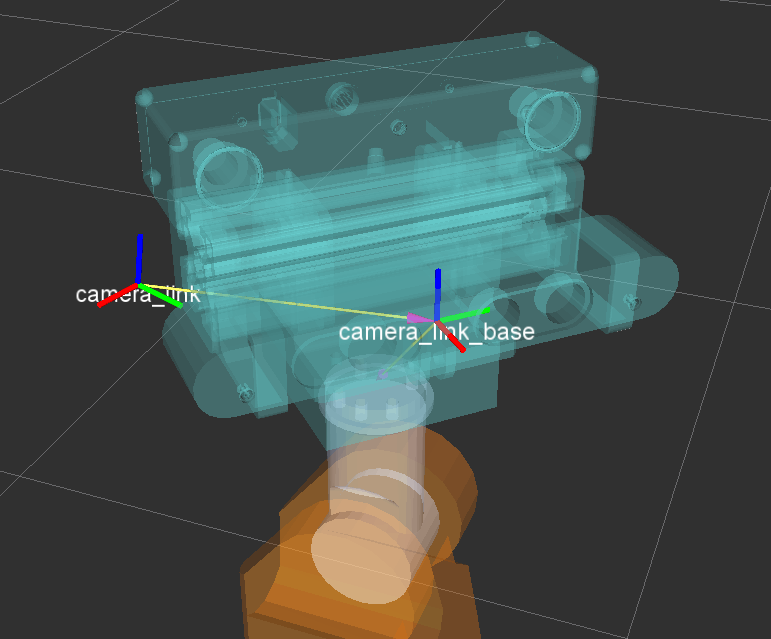
\includegraphics[width=\textwidth]{graphics/08_resultsdiscussion/calibration_result_rviz1.png}
			\end{center}
        \end{subfigure}
        \begin{subfigure}[b]{0.4\textwidth}
        \begin{center}
			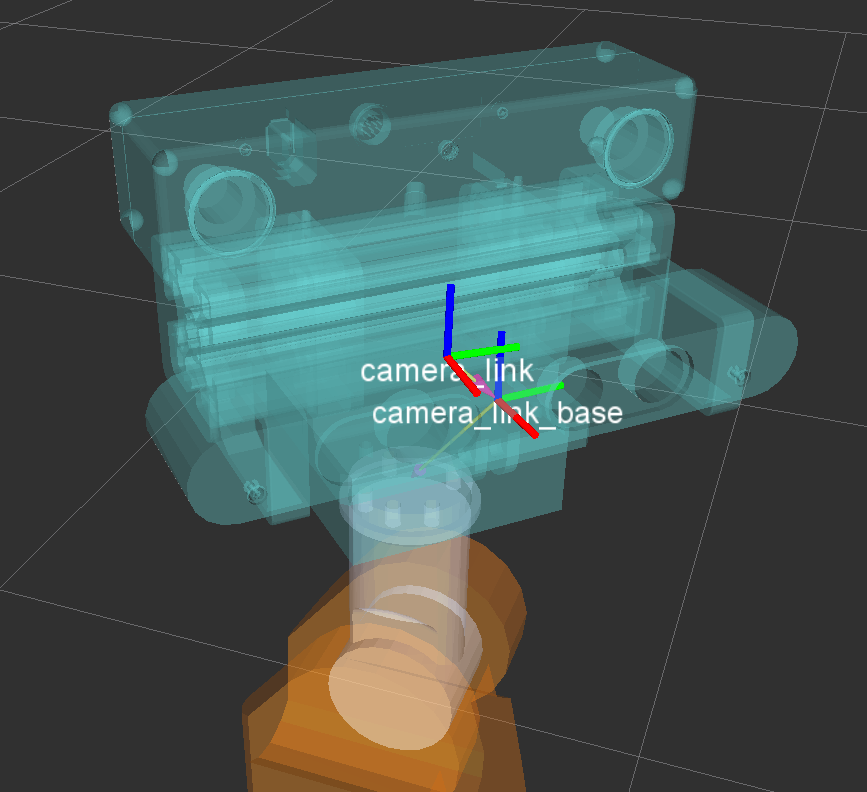
\includegraphics[width=0.9\textwidth]{graphics/08_resultsdiscussion/calibration_result_rviz2.png}
			\end{center}
        \end{subfigure} 
		\caption{Shows two examples of the calibration. One faily realistic (right) and the other way off.}\label{fig:calibration_tf}
\end{figure}

It is assumed that the reason for the inconsistency is some underlying factors, that have yet to be discovered. Visualising the stereo data in the robot cell shows lots of noise (figure \ref{fig:stereo_vis}) which could be part of the reason. 

\begin{figure}[htb]
	\centering
        \begin{center}
			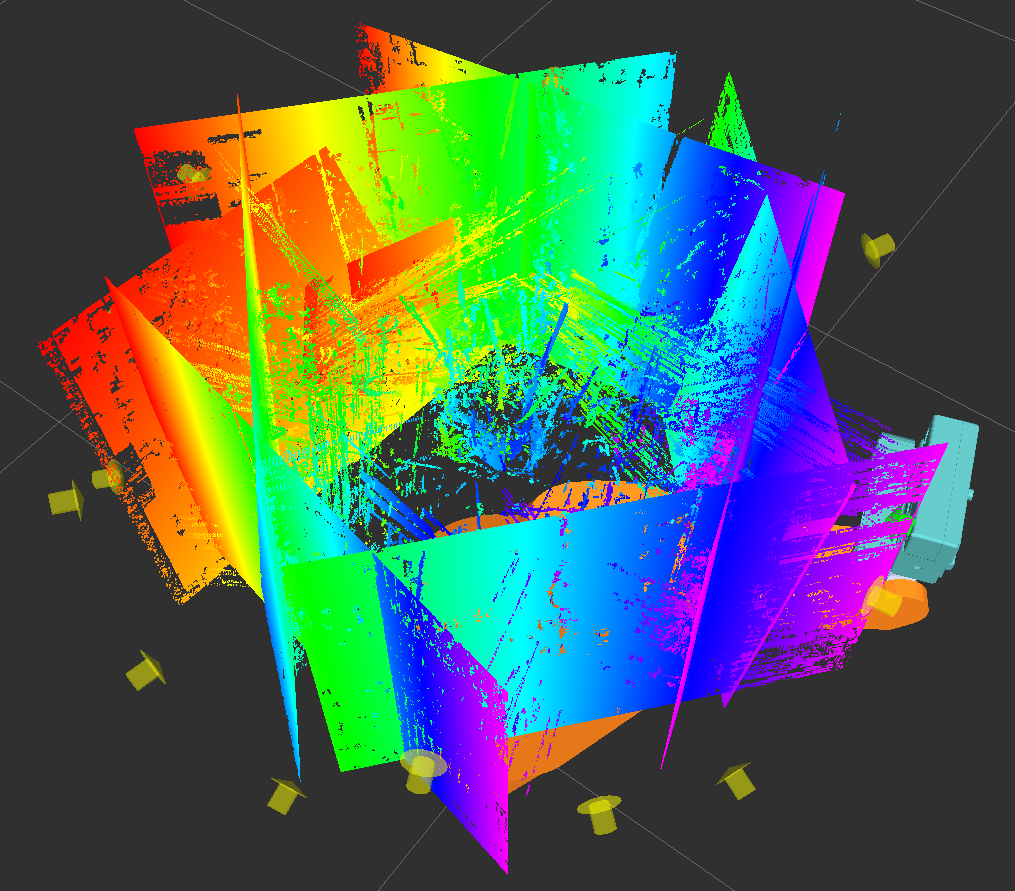
\includegraphics[width=0.9\textwidth]{graphics/08_resultsdiscussion/stereo_data_in_robotscene.png}
		\end{center}
		\caption{Shows the individual point clouds from the vision component, visualised in the robot scene.}\label{fig:stereo_vis}
\end{figure}